\documentclass[12pt,a4paper]{report}
%\usepackage[a4paper, total={6in, 8in}]{geometry}
\usepackage{geometry}
 \geometry{
 top=25mm,
 }
%\usepackage[showframe]{geometry}
\usepackage{titlesec}
%\usepackage{titletoc,tocloft}
\usepackage[english]{babel}
\usepackage[T1]{fontenc}
\usepackage{mathptmx}
%\usepackage{newtxmath,newtxtext}
%\usepackage[utf8x]{inputenc}
\usepackage{amsmath}
\usepackage{graphicx}
\graphicspath{ {images/} }
\usepackage[colorinlistoftodos]{todonotes}
\usepackage[yyyymmdd]{datetime}
\usepackage{tikz}
\usetikzlibrary{calc}
\usepackage{sectsty}
\usepackage{float}
%\usepackage[tocflat]{tocstyle}
%\usetocstyle{standard}
%\usepackage[table,xcdraw]{xcolor}
\sectionfont{\fontsize{18pt}{15}\selectfont}
\usepackage{tocloft}
\usepackage{subcaption}
%\renewcommand{\cftsecleader}{\cftdotfill{\cftdotsep}}
%add page no
%\addtocontents{toc}{{\bfseries \hfill Page No.\bigskip\par}}

%\setlength{\cftsubsecindent}{2cm}
%\setlength{\cftsubsubsecindent}{4cm}

\titleformat
{\chapter} % command
[display] % shape
{\bfseries\Large} % format
{\centering Chapter \thechapter} % label
{0.5ex} % sep
{
%    \rule{\textwidth}{1pt}
%    \vspace{1ex}
\Large 
    \centering
    \MakeUppercase
} % before-code
\titlespacing*{\chapter}{0pt}{-50pt}{30pt}


%\tableofcontents


\begin{document}
\pagenumbering{roman}
\linespread{1.3}
%\addcontentsline{toc}{section}{Unnumbered Section}\
\addcontentsline{toc}{section}{\textbf{Approval}}
\fontsize{13pt}{12}\selectfont{Approval of the Department of Electronic \& Telecommunication Engineering}\\[2cm]

\begin{table}[h]
\begin{tabular}{cc}
 & \hspace{8cm}..........................................                                                                               \\
 & \begin{tabular}[c]{@{}c@{}}\hspace{8cm}Head, Department of Electronic \&\\ \hspace{8cm}Telecommunication Engineering\end{tabular}
\end{tabular}
\end{table}
\vspace{2.5cm}
\noindent This is to certify that I/we have read this project and that in my/our opinion it is fully adequate, in scope and quality, as an Undergraduate Graduation Project.\\[1cm]
Supervisors:\\[0.5cm]
Dr. Ranga Rodrigo\\[1cm]
Signature: ......................\\[1cm]
Dr. Ajith Pasqual\\[1cm]
Signature: ......................\\[1cm]
Dr. Peshala G. Jayasekara\\[1cm]
Signature: ......................\\[2cm]
Date: ......................\\


\newpage
\addcontentsline{toc}{section}{\textbf{Declaration}}
\begin{center}
\fontsize{18pt}{12}\selectfont{\textbf{Declaration}}
\end{center}
\fontsize{12pt}{12}\selectfont
This declaration is made on October 5, 2017.\\[1cm]
\textbf{Declaration by Project Group}\\
We declare that the dissertation entitled People Counting and Tracking with Xilinx ZC702 Evaluation Kits and the work presented in it are our own. We confirm that:
\begin{itemize}
\item this work was done wholly or mainly in candidature for a B.Sc. Engineering degree at this university,
\item where any part of this dissertation has previously been submitted for a degree or any other qualification at this university or any other institute, has been clearly stated,
\item where we have consulted the published work of others, is always clearly attributed,
\item where we have quoted from the work of others, the source is always given. With the exception of such quotations, this dissertation is entirely our own work,
\item we have acknowledged all main sources of help.
\end{itemize}
\vspace{1cm}
\begin{table}[h]
\begin{tabular}{cccc}
........................... &&& \hspace{5cm}...........................  \\
Date                        &&& \hspace{5cm}R.V.C.N Abeyrathne (130008K) \\[1cm]
                            &&& \hspace{5cm}...........................  \\
                            &&& \hspace{5cm}D.L Dampahalage (130093M)    \\[1cm]
                            &&& \hspace{5cm}...........................  \\
                            &&& \hspace{5cm}H.A.S.P Gunasekara (130183N) \\[1cm]
                            &&& \hspace{5cm}...........................  \\
                            &&& \hspace{5cm}W.M.D.K Weerakoon (130633V) 
\end{tabular}
\end{table}
\newpage
\noindent \textbf{Declaration by Supervisors}\\[0.5cm]
We have supervised and accepted this dissertation for the submission of the degree.\\[1cm]
\begin{table}[h]
\begin{tabular}{cc}
........................... & \hspace{5cm}........................... \\
Dr. Ranga Rodrigo           & \hspace{5cm}Date                        \\[1cm]
........................... & \hspace{5cm}........................... \\
Dr. Ajith Pasqual           & \hspace{5cm}Date                        \\[1cm]
........................... & \hspace{5cm}........................... \\
Dr. Peshala G. Jayasekara   & \hspace{5cm}Date                       
\end{tabular}
\end{table}
\newpage
\addcontentsline{toc}{section}{\textbf{Abstract}}
\begin{center}
\fontsize{18pt}{18}\selectfont{\textbf{Abstract\\[1cm]
People Counting and Tracking with Xilinx ZC702\\
Evaluation Kits}}\\[0.5cm]
\fontsize{12pt}{12}\selectfont{Group Members: R.V.C.N Abeyrathne, D.L Dampahalage, H.A.S.P Gunasekara, W.M.D.K Weerakoon}\\[0.25cm]
Supervisors: Dr. Ranga Rodrigo, Dr. Ajith Pasqual, Dr. Peshala G. Jayasekara
\end{center}
\textit{Keywords}: FPGA,ZYNQ-7000, people counting, multi-camera, multiple people tracking, particle filters, gaussian mixture models\\[0.5cm]
In the contemporary society making correct decisions is vital for any business organization to stay on par with competitors. For that intent identifying and understanding the
customers is a must. Tapping into the customers$'$ subconscious is the preeminent way of making correct business decisions and for that an organization should track and analyze customer behavior.\\
As a solution to this problem, we propose a scalable multi-camera people tracking system for a large department store like environment. The main focus of this project is to implement an end to end system for multi-camera people tracking with business intelligence.
Novelty of this system from contemporary multi-camera people tracking systems is the introduction of leaf node processing, where part of the processing is done in a hardware system close to the camera. By this way we could achieve the scalability required for a large department store like environment and reduce bandwidth usage in such systems.\\
This proposed system comprises of leaf nodes, central server and the web server. Leaf nodes are integrated close each camera. We use Zynq SoCs for leaf nodes and these devices read video frames from the cameras, detects people for each frame using GMM based background subtraction, calculate color histogram features for each detected person and sends the bounding boxes and features to the server using UDP.\\
A central server will receive this information from each leaf node and do people tracking by using particle filters and hungarian algorithm for data association. Multi-camera tracking is also achieved by means of homography based method and a graph algorithm. Real time tracking and heatmaps are generated in the server GUI.\\
Finally business intelligence software hosted in a web server, where real time people tracking for the whole store, heatmaps for desired time period, people count graphs for desired time period and real time people count graphs are implemented.\\
Therefore by the introduction of leaf node processing we achieve a scalable system since the processing power required at the central server is reduced. We achieve a low power system for leaf nodes by using Zynq SoCs and we reduce the bandwidth usage since we only send the bounding boxes and features for tracking to the server.


\newpage
\addcontentsline{toc}{section}{\textbf{Acknowledgments}}
\begin{center}
\fontsize{18pt}{18}\selectfont{\textbf{Acknowledgments}}
\end{center}
\vspace{1cm}
We would like to express our deepest appreciation and sincere gratitude to our project supervisors, Dr. Ajith Pasqual, Dr. Ranga Rodrigo and Dr. Peshala Jayasekara of Department of Electronic and Telecommunication Engineering of University of Moratuwa, for their guidance and constant supervision as well as for providing necessary information regarding the project.\\
\par We would like to thank ParaQum Technologies for their guidance and support given to us during the project.
We are indebted to our final year project coordinator, Dr. Anjula Silva for his counsel regarding the project.
We would also like to take this opportunity to thank Ms. Salgado for her advices on compiling a finer report.
We would like to acknowledge with much appreciation the non-academic staff of the department who gave us their fullest support in providing necessary laboratory facilities.\\
\par Finally, our thanks and appreciations also goes out to our batch mates who helped in numerous ways to make this endeavor a success.
\newpage
\titleformat*{\section}{\centering\bfseries\Large}
\tableofcontents
\titleformat*{\section}{\bfseries\Large}
\newpage
\addcontentsline{toc}{section}{\textbf{List of Figures}}
\listoffigures
\newpage
\addcontentsline{toc}{section}{\textbf{List of Tables}}
\listoftables
\newpage
\addcontentsline{toc}{section}{\textbf{Acronyms and Abbreviations}}
\begin{center}
\fontsize{18pt}{18}\selectfont{\textbf{Acronyms and Abbreviations}}
\end{center}
\vspace{0.75cm}

\begin{table}[H]
\centering
\begin{tabular}{ll}
FPGA & Field Programmable Gate Array \\
GMM & Gaussian Mixture Models\\
PCA & Principal Component Analysis \\
YOLO                     & You Only Look Once                                \\
IP                       & Intellectual Property                             \\
SoC                      & System on Chip                                    \\
RTL                      & Register Transfer Level                           \\
AXI                      & Advanced eXtensible Interface                      \\
HLS                      & High Level Synthesis                              \\
UIO                      & Userspace Input/Output                            \\
REST                     & Representational State Transfer                   \\
API                      & Application Programming Interface                 \\
AJAX                     & Asynchronous JavaScript ond XML                   \\
JSON                     & JavaScript Object Notation                        \\
UDP                      & User Datagram Protocol                            \\
TCP                      & Transmission Control Protocol                     \\
URL                      & Uniform Resource Locator                          \\
SDRAM                    & Synchronous Dynamic Random Access Memory          \\
DDR                      & Double Data Rate                                 
\end{tabular}
\end{table}
\newpage
\pagenumbering{arabic}
\setcounter{page}{1}

\chapter{\textbf{Introduction}}
In the contemporary society making correct decisions is vital for any business organization to stay on par with competitors. For that intent identifying and understanding the customers is a must. Tapping into the customer's’ subconscious is the preeminent way of making correct business decisions and for that an organization should track and analyze customer behavior.\vspace{0.3cm}
\par For retail stores and shopping malls gathering customer insight could be done by analyzing the
behavior of day to day customers. However counting and keeping track of customers is a tedious task for a large store structure by just employing a number of cameras and a manual
System.\vspace{0.3cm}

As a possible solution, we have proposed a people tracking and counting system adaptable to any large scale store structure. The objective of this project is to develop a system that is able to process multiple video streams obtained through separate cameras mounted on a store structure in order to track customers and generate business intelligence.

There have been several systems which handle multi camera people tracking introduced in the past decade. All these systems incorporate a central server which will receive all the frames from all the cameras to handle the people detection and tracking tasks real-time. This is not scalable in a large environment unless the central server has enough processing power. Solution to this problem is to do part of the processing close to the camera which we define as leaf node processing.\vspace{0.3cm}

We propose a system which utilizes a FPGA + ARM Processor at the leaf node for the people detection. This system will then send the information to the central node for Multi-Camera Tracking, thereby reducing the processing power required at the central server. Also  the system is only sending the bounding boxes and features for tracking which reduces the bandwidth usage in such systems.\vspace{0.3cm}

Scope of this project is to implement a scalable end to end system for Multi-Camera People Tracking utilizing a Zynq SoC for leaf node processing. Thereby we use an FPGA + ARM processor for leaf node processing, a central server for multi-camera people tracking and a web server for generating business intelligence.\vspace{0.3cm}

People Detection in FPGA is an aspect that has been researched by many over the years. For example  [2] suggests a FPGA based embedded platform for people detection using Gaussian Mixture Models and [3] suggests a similar system for people detection using Histogram of Features. \vspace{0.3cm}
Multi-Camera People Tracking systems is also a field which has been researched over the years. [4] suggests a multi-camera surveillance system implemented with background subtraction for detection and color features for tracking. [6] suggests another multi camera people tracking system which uses particle filters for tracking on the ground plane.\vspace{0.3cm}

Major drawback of these systems is the scalability. When the number of cameras increase, the bandwidth usage for sending video frames to the central server will be increased and the processing power required at the central server will increase. This raises the requirement for processing video frames close to the camera which is defined as leaf node processing.\vspace{0.3cm} 

In this proposed system by using a FPGA + ARM processor we have achieved leaf node processing of people detection at a lower power and also enable the scalability and lower bandwidth requirement. 

\chapter{Literature Review}
In this project main focus was to implement an end to end system for Multi-Camera People Tracking System and to use this system to generate business intuition. As explained earlier we use the technique of leaf node processing to achieve a scalable, low power, low bandwidth required system.\vspace{0.3cm} 

There are several challenging tasks in implementing this system. One is people detection in FPGA. There are various ways to achieve this. One way is to use a blob detection algorithm as used by Vicente, Alfredo Gardel, et al. [1] in 2009.They have done background subtraction followed by contour detection to select head candidates for videos obtained using overhead cameras and they have implemented people detection part in a low cost FPGA (spartan3).\vspace{0.3cm}

Feature based methods are also another way to do people detection. In these methods a set of features are calculated around a window and some kind of machine learning algorithm is used to train a classifier that can classify each window into "contains a person" and "not contains a person". One such method is Histogram Oriented Gradient (HoG) based method suggested by Dalal, Navneet, and Bill Triggs. [2] in 2005. A variation of HoG is implemented on FPGA by Negi, Kazuhiro, et al. [3] in 2011.\vspace{0.3cm}

Another approach that can be used for people detection is to utilize a neural network. If we can come up with a suitable neural network architecture, this method has the potential to outperform all the other methods mentioned earlier. There are several open source implementations of such architectures available. One such architecture is given by Redmon, Joseph, et al. [4] in 2016. Their work has made a huge leap in object detection space. Due to its success their architecture is utilized by many people. Challenge though in using this approach is the complexity of implementing a convolutional neural network in an FPGA.  Implementing a CNN architecture in FPGA with the available resources and to achieve real time processing is an immense challenge. \vspace{0.3cm}

We used a background subtraction based method for people detection in the proposed system. Though we considered using either HoG or CNN, as our focus was to implement the end end architecture for multi-camera people tracking with leaf node processing, background subtractions deemed to be a feasible solution. We could improve the existing system by implementing either HoG or CNN as a future improvement.\vspace{0.3cm}

Other major challenge we have is people tracking based on our detections. There are many traditional approaches to this such as tracking using kalman filter and assigning detections to tracks using the Hungarian algorithm. But multi target tracking also can be formulated as a discrete-continuous optimization problem [5]. Andriyenko, Anton, Konrad Schindler, and Stefan Roth [5] in 2012 have considered data association as a discrete optimization problem with label costs. And they have posed trajectory estimation as a continuous fitting problem with closed form solutions. And there method has performed well on some known data sets.\vspace{0.3cm}

Other major challenge that we face is, how to extend multiple target tracking into a multi camera framework. There are some research papers discussing this issue. Tang, Nick C., et al. [6] in 2015 suggest a two pass regression framework to solve this challenge. First pass regression predicts the people count based on the features calculated from intra-camera video frames. And then the second pass is based on the conflicts between the prediction derived from multiple views. They have formulated this as a transfer learning problem. Yang, Tao, et al. [7] in 2007 discusses another method to do this. In this approach first they do single camera tracking and they transform these tracked paths into a global coordinate system. Then by using their multi camera handoff algorithm, they can track people across multiple cameras. Here they calculate a match score for an object appearing in a camera under overlapping or non overlapping conditions for all tracks under all cameras. The track having the maximum score is selected.\vspace{0.3cm}

By going through the available literature we were able to get an insight of the scope of our project. We identified some potential solutions for the challenges we have. We were also able to identify that implementing the overall system architecture for multi-camera people tracking with leaf node processing will be a novel contribution. 


\chapter{Methodology}
\section{Introduction}
In this project we have designed and implemented an end to end multi camera people counting and tracking system based on Xilinx ZC702 development board. In this implementation we have considered the possibility of using leaf node processing to develop a scalable solution for multi camera people tracking. In this chapter we present the underline methodology of our system in detail.
In order to give the reader a gradual walkthrough of our project we will explore each component of our system separately. First we will give an overview of the basic system. Then we will explore in detail the each component of our system. 

\section{Overall Architecture}
\begin{figure}[H]
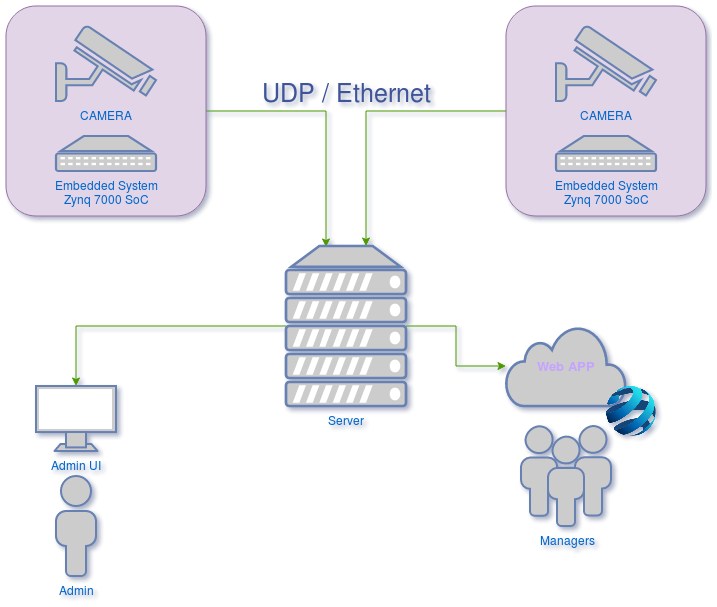
\includegraphics[width=10cm]{overall_block.png}
\centering
\caption{Overall block diagram of the end-to-end system}
\label{overall}
\end{figure}

Figure \ref{overall} shows the overall architecture of our system. It mainly consist of 3 components, namely,
An embedded system closer to the camera (Leaf node)
People tracking applications running on a server 
Business intelligence generation and displaying interfaces. 

We will explore each of the above components separately in the following sections.

\section{Embedded System (Leaf Node)}
Generally the term 'leaf node' is used for a system placed at the edge or bottom of a hierarchical network (of systems). In our system, leaf node is the embedded system connected to the camera.  
This embedded system  is responsible for capturing live video frames from the camera and preprocessing before sending into the central server. Objective of preprocessing on the leaf node is to reduce the required bandwidth of the network to send information (video in this case) to the central server and to reduce the processing done one the central server in a scalable manner. 
In a large system consisting of few hundreds of cameras, reduction of the bandwidth required and the processing power of the central system for each camera makes a big difference in the central system processing and bandwidth requirements, making the system more scalable.  

In our prototype system, leaf node consists of a web camera connected to a Xilinx ZC702 development board and its responsible for doing people detection of the live video feed and feature calculation of the detected people. Implementations of the people detection and feature calculation algorithms are explained in detail in later sections. These calculated features of the detected people are then sent to the central server via a custom application layer protocol based on User Datagram Protocol (UDP) / Internet Protocol (IP) over Ethernet.

Following sections provide an overview about the feature of Xilinx ZC702 board and ZYNQ-7000 All Programmable (AP) System on Chip (SoC).

\subsection{Xilinx ZC702 Board}
Xilinx ZC702 board, shown in Figure \ref{board}, is a development board manufactured by Xilinx targeting embedded hardware (FPGA) design development. This board consists of a ZYNQ-7000 AP SoC with various other peripherals. Key features and peripherals of Xilinx ZC702 is listed below.




\begin{itemize}
\item Zynq-7000 SoC
\item 1GB DDR3 Component Memory
\item Enabling serial connectivity with USB OTG, UART, IIC, CAN Bus
\item Ethernet which supports 10-100-1000 Mbps transfer rates
\item HDMI interface
\item FPGA Mezzanine Card (FMC) interface
\item Onboard Secure Digital (SD) card reader
\end{itemize}


\begin{figure}[H]
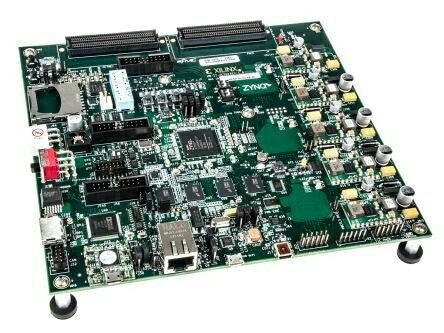
\includegraphics[width=10cm]{zc702.jpg}
\centering
\caption{Xilinx ZC702 Development Board}
\label{board}
\end{figure}


Features of the onboard ZYNQ-7000 SoC and usage of it in our project is explained in following sections.

\subsection{ZYNQ-7000 SoC}
ZYNQ-7000 SoC consists of a Xilinx XC7Z020-CLG484-1 FPGA and two ARM Cortex-A9 core processors. Block diagram in figure \ref{zynq} shows how the Programmable Logic and the Processing System is connected inside the ZYNQ-7000 SoC.

\begin{figure}[H]
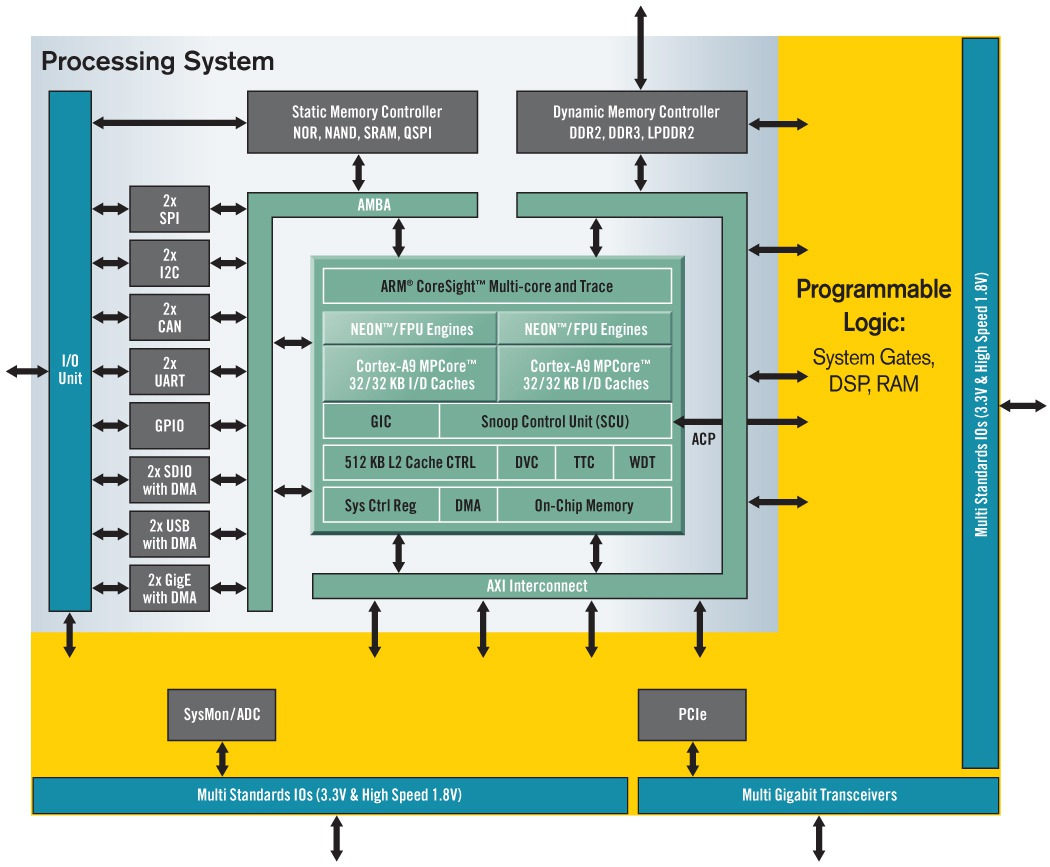
\includegraphics[width=10cm]{zynq.jpg}
\centering
\caption{Internal architecture of ZYNQ-7000 SoC}
\label{zynq}
\end{figure}

In our implementation, we have installed a lightweight Linux distribution on dual ARM processors in ZYNQ-7000 SoC. Reasons for installing Linux and its usage is explained in a latter section.


\section{Design Flow for ZYNQ-7000 based Embedded System}
We used the standard Xilinx toolchain for developing an embedded system for designing and implementing our leaf node system. Figure \ref{design} shows a block diagram of the design flow with the design tools we used.

\begin{figure}[H]
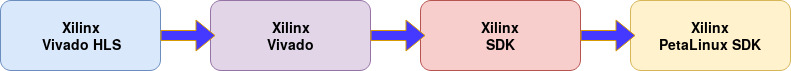
\includegraphics[width=13cm]{design.jpg}
\centering
\caption{Design flow block diagram for ZYNQ-7000 based embedded system}
\label{design}
\end{figure}

Brief description about the usage of each tool in the design flow is included in the following subsections.

\subsection{Vivado HLS}
HLS stands for High Level Synthesis. Task of Vivado HLS is to synthesize a function developed using a high level language (C, C++ and SystemC) into a RTL design (Hardware Descriptive Language Code) of an IP Core. 

\subsection{Vivado}
IP cores designed using Vivado HLS are then imported to Vivado for designing the overall architecture. This is the tool where we decide how the PL and PS parts of ZYNQ SoC is connected (which type of AXI protocol). After overall system is designed, its synthesized and implemented on the target device. As an output of this process, bit-stream file and hardware description (HDF) file is generated.

\subsection{Xilinx SDK}
HDF file generated is then imported to Xilinx SDK for testing the functionality of implemented hardware. Xilinx SDK has options for testing the hardware on the target device by writing a simple C/C++ application code for testing the functionality of the implemented hardware.

\subsection{PetaLinux SDK}
After confirming the functionality of the hardware on the target device, HDF file is then imported to a PetaLinux SDK project for generating the Linux boot files for the custom hardware. Enabling the required kernel modules and editing the device tree to enable hardware peripheral access is done here. More details about running Linux on ZYNQ PS is explained in the next section.

\section{Installing Linux on ZYNQ-7000}
Lightweight customized Debian Linux distribution was installed on ARM processors of ZYNQ SoC. When it comes to running applications on PS of ZYNQ, there are two primary options,

\begin{enumerate}
\item Running a Linux distribution 
\item Running the application in baremetal mode (Using the basic drivers provided by Xilinx)
\end{enumerate}

\noindent We choose to install and run a Linux distribution based on the following reasons,
\begin{itemize}
\item Complete and working protocol stacks for communication protocols (Ethernet, UART)
\item Readily available device drivers for interfacing various hardware (USB web camera, USB tethering)
\item Root file system stored in the SD card (Usually bare-metal application use onboard RAM to store data at run time, which will be destroyed after turning off the board)
\item Linux comes with a package manager that can be used to install almost any third party Linux compatible software package (Python, C++ compilers).
\end{itemize}

\section{People Detection and Feature Calculation Implementation on ZYNQ-7000 SoC}


\subsection{IP core implementation on ZYNQ PL}

\subsubsection{Gaussian Mixture Model Background Subtraction IP Core}

\subsubsection{Feature Calculation IP Core}

\subsection{IP Core drivers, Morphological Operations and Communication Protocol Implementation on ZYNQ PS}

\subsubsection{Linux Drivers for controlling IP cores}

\subsubsection{People Detection from Background Subtracted Binary Mask}

\begin{figure}[H]
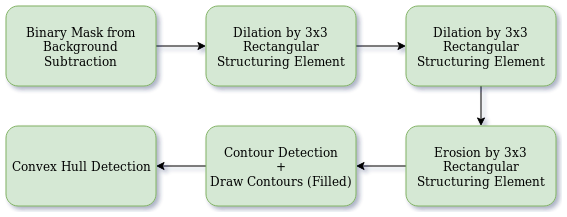
\includegraphics[width=13cm]{morphology.png}
\centering
\caption{Block diagram of the morphological operation flow to detect people from background subtracted binary mask}
\label{morphology}
\end{figure}

Once the background subtracted binary mask is obtained a set of operations are performed as shown in figure \ref{morphology} to enhance the binary image for object detections. 
First a set of morphological operations are performed to clean out the image as necessary. Since the quality of the background model can vary due to various environmental conditions, background subtraction will not give a cleanly filled blob for the shape of a person. There will be a lot of black pixels on the boundary as well as inside the shape of a person. We can use the morphological operation ‘closing’ to fill out these holes. It is essentially two dilations followed by an erosion. Structuring element used here is a 3x3 rectangle. We have tested out several alternatives for the kernel but this kernel size and shape gave the best results for the sequences of images we have tested. Therefore we used it in our final implementation. The results of morphological operations for a test images is shown in figure \ref{fig:sfig3}, \ref{fig:sfig4} and \ref{fig:sfig5}.

\begin{figure}
\begin{subfigure}{.5\textwidth}
  \centering
  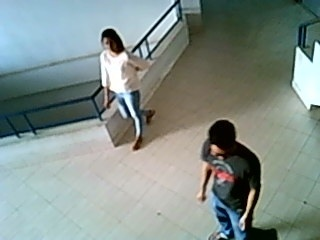
\includegraphics[width=.8\linewidth]{morphology/original.jpeg}
  \caption{Original image}
  \label{fig:sfig1}
\end{subfigure}%
\begin{subfigure}{.5\textwidth}
  \centering
  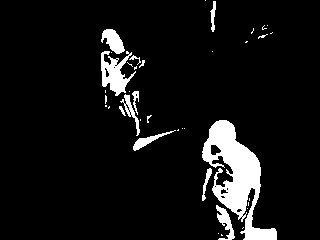
\includegraphics[width=.8\linewidth]{morphology/bgsub.jpeg}
  \caption{Background subtracted binary mask}
  \label{fig:sfig2}
\end{subfigure}\\
\begin{subfigure}{.5\textwidth}
  \centering
  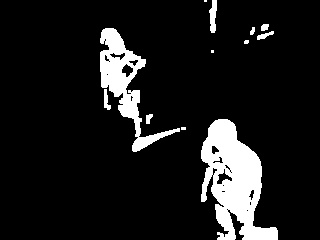
\includegraphics[width=.8\linewidth]{morphology/dilate1.jpeg}
  \caption{Dilation performed on the binary mask}
  \label{fig:sfig3}
\end{subfigure}%
\begin{subfigure}{.5\textwidth}
  \centering
  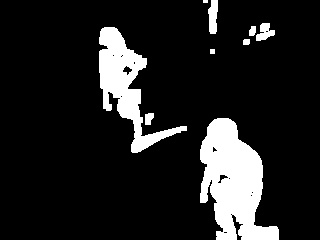
\includegraphics[width=.8\linewidth]{morphology/dilate2.jpeg}
  \caption{Twice dilated}
  \label{fig:sfig4}
\end{subfigure}\\
\begin{subfigure}{.5\textwidth}
  \centering
  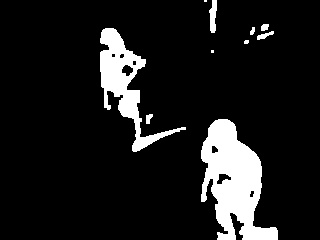
\includegraphics[width=.8\linewidth]{morphology/errode.jpeg}
  \caption{Twice dilated and eroded}
  \label{fig:sfig5}
\end{subfigure}%
\begin{subfigure}{.5\textwidth}
  \centering
  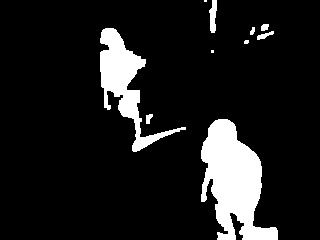
\includegraphics[width=.8\linewidth]{morphology/shape.jpeg}
  \caption{Contour detection and drawing the filled contours taking \ref{fig:sfig5} as input}
  \label{fig:sfig6}
\end{subfigure}\\
\centering
\begin{subfigure}{.8\textwidth}
  \centering
  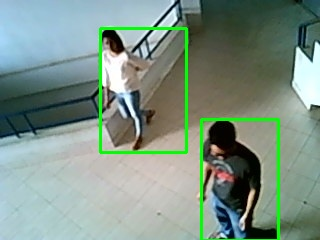
\includegraphics[width=.5\linewidth]{morphology/detections.jpeg}
  \caption{Detecting bounding boxes using convex hull detection}
  \label{fig:sfig7}
\end{subfigure}
\caption{Results of morphological operations for a test image}
\label{fig:fig}
\end{figure}

Morphological operations will give a cleaner image compared to the original background subtracted image. Next contour detection is applied to the output image resulting from morphological operations. We have used inbuilt functions of opencv for this. They have implemented contour detection based on Suzuki’s [7] border following algorithm. Then again using inbuilt functions of opencv we fill out these contours. It will completely fill the shape of the person. The result of this operation for a test image is shown in figure \ref{fig:sfig6}.

Next step in this process is to detect the bounding box surrounding the blob of a person. For this we use opencv inbuilt function for convex hull detection. A convex hull is the smallest polygon enclosing a set of points. Opencv’s implementation is based on the algorithm proposed by Sklansky [8]. After this process we obtain a set of bounding boxes corresponding to people detected. Resulting bounding boxes for a test image is shown in figure \ref{fig:sfig7}.

\subsection{False Positive Reduction}
Although the above process is able to detect people from an image, it also detects a lot of unwanted blobs due to various reasons such as reflections caused by background surfaces, imperfections of background modeling, etc. Therefore we need to utilize a method to reduce number of these false positives. Our initial approach was to select the bounding boxes satisfying a set of conditions as follows and reject all the other detections.
\begin{itemize}
\item Width of bounding box(w) > TW
\item Height of bounding box(h) > TH
\item TAR1 > Aspect ratio(w/h) > TAR2
\item TCA1 > Contour Area > TCA2
\end{itemize}
Here TW, TH, TAR1, TAR2, TCA1 and TCA2 are constants that are chosen arbitrarily. Initially we tuned up these constants manually by looking at the results. But this was a tedious task and this has to be redone once the camera position is changed. Therefore we explored the possibility of machine learning based automatic way to do this.

\noindent We selected a few features of the bounding boxes into consideration as follows:
\begin{enumerate}
\item Width
\item Height
\item Bounding box area
\item Aspect Ratio (Width / Height)
\item Contour Area
\item Diagonal Length
\end{enumerate}

\begin{figure}[H]
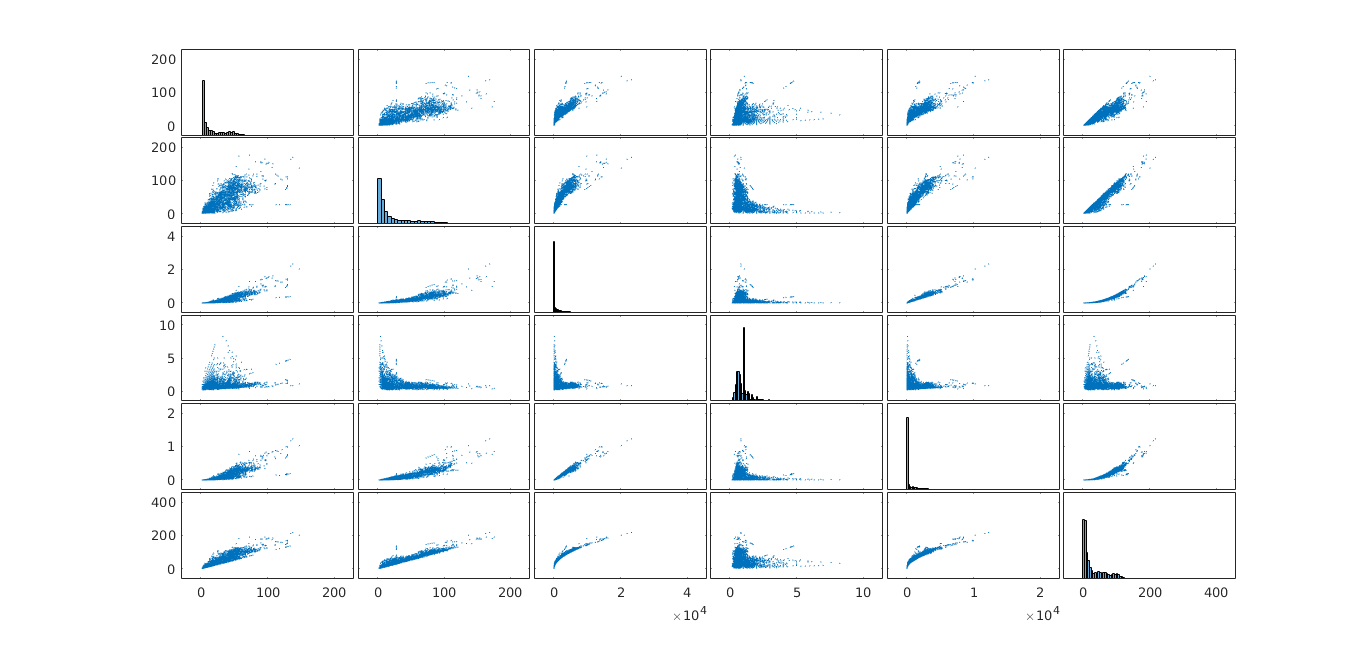
\includegraphics[width=\textwidth]{pca/scatter_plots_pca.png}
\centering
\caption{Scatter plot matrix for the 6 features collected from running our object detection on a sample video}
\label{pca1}
\end{figure}


We can see from the scatter plots above that most of the above features are highly correlated. Therefore we can use Principal Component Analysis to perform dimensionality reduction of the feature space. The percentage of variance explained by each principal component was obtained as follows.

\begin{table}[]
\centering
\caption{Percentage of variance along each pricipal component}
\label{pca-table}
\begin{tabular}{|c|c|}
\hline
\textbf{Principal Component} & \textbf{Percentage of Variance Explained} \\ \hline
1                            & 99.4509                                   \\ \hline
2                            & 0.5401                                    \\ \hline
3                            & 0.0063                                    \\ \hline
4                            & 0.0019                                    \\ \hline
5                            & 0.0000                                    \\ \hline
6                            & 0.0000                                    \\ \hline
\end{tabular}
\end{table}

We can see that only the first two principal components give a significant contribution. Even the 2d principal component is less significant compared to the 1st principal component. We can further see this in figure \ref{pca2}.

\begin{figure}[H]
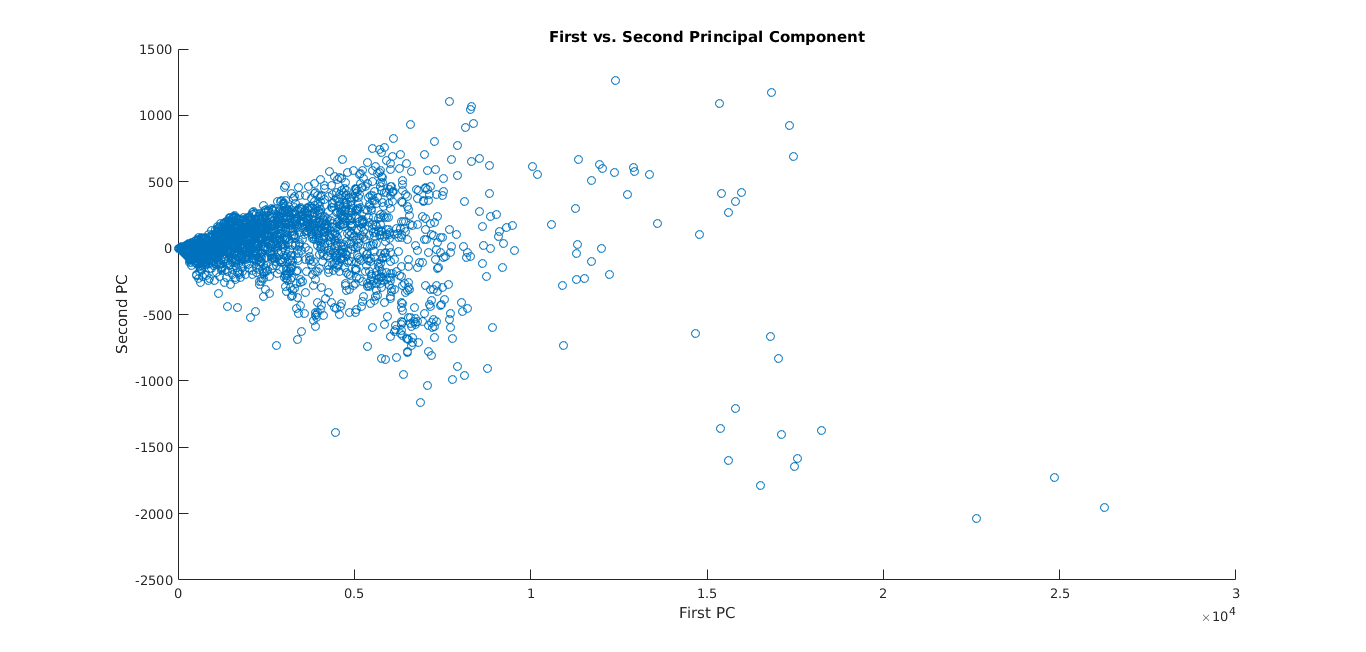
\includegraphics[width=\textwidth]{pca/1_2_pca.png}
\centering
\caption{First Vs. second pricipal component}
\label{pca2}
\end{figure}

\noindent Therefore it is justifiable only to select the first principal component into consideration. 


\begin{figure}[H]
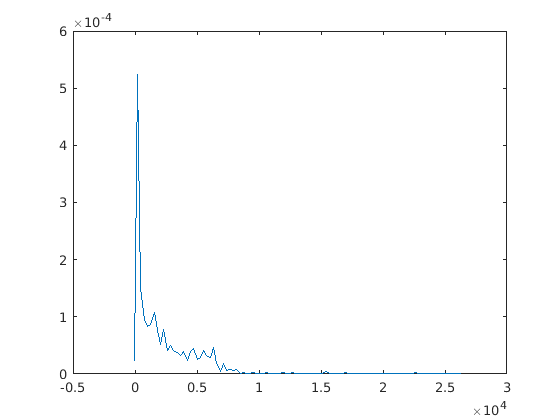
\includegraphics[width=\textwidth]{pca/density.png}
\centering
\caption{Density of the first principal component}
\label{pca3}
\end{figure}

Next we looked at the kernel density estimate of the first principal component as shown in figure \ref{pca3}. We can approximate this with a bimodal distribution. Therefore the problem reduces to finding the optimum threshold for this bimodal distribution. We used Otsu’s [9] thresholding algorithm to find this threshold.

We utilized this framework for false positive reduction of the detections. Once we tested out this with several video sequences taken from different camera angles we found out that this method indeed gives better results as analysis suggested. Figure \ref{pca4:pca4} shows the results of PCA based false positive reduction.

\begin{figure}
\begin{subfigure}{.5\textwidth}
  \centering
  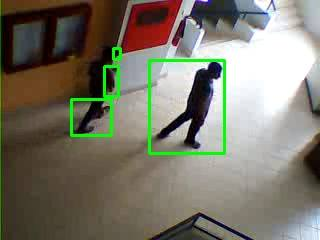
\includegraphics[width=.8\linewidth]{pca/fals_positives.jpg}
  \caption{Raw bounding boxes detected}
  \label{pca4:1}
\end{subfigure}%
\begin{subfigure}{.5\textwidth}
  \centering
  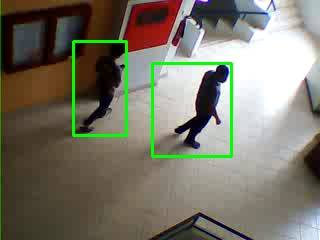
\includegraphics[width=.8\linewidth]{pca/false_positives_eliminated.jpg}
  \caption{With false positive reduction}
  \label{pca4:2}
\end{subfigure}
\caption{Results of PCA based false positive elimination algorithm}
\label{pca4:pca4}
\end{figure}

When applying this method the system should first undergo a training stage where raw detection features are collected. Then coefficients of the first principal component is determined using this dataset. Then the optimum threshold is determined. This whole process was implemented in code so that system can automatically learn to reduce false positives. In the normal mode of operation the system directly uses these calculated coefficients and threshold for false positive reduction.


\chapter{Results}


\subsection{Discussion}



\newpage
%\section*{\textbf{References}}
\addcontentsline{toc}{section}{References}
\begin{thebibliography}{10}

\bibitem{1}
Vicente, Alfredo Gardel, et al. "Embedded vision modules for tracking and counting people." \textit{IEEE Transactions on Instrumentation and Measurement} 58.9 (2009): 3004-3011.

\bibitem{2}
Dalal, Navneet, and Bill Triggs. "Histograms of oriented gradients for human detection." Computer Vision and Pattern Recognition, 2005. CVPR 2005. \textit{IEEE Computer Society Conference on}. Vol. 1. IEEE, 2005.

\bibitem{3}
Negi, Kazuhiro, et al. "Deep pipelined one-chip FPGA implementation of a real-time image-based human detection algorithm." \textit{Field-Programmable Technology (FPT), 2011 International Conference on}. IEEE, 2011.

\bibitem{4}
Redmon, Joseph, et al. "You only look once: Unified, real-time object detection." \textit{Proceedings of the IEEE Conference on Computer Vision and Pattern Recognition}. 2016.

\bibitem{5}
Andriyenko, Anton, Konrad Schindler, and Stefan Roth. "Discrete-continuous optimization for multi-target tracking." \textit{Computer Vision and Pattern Recognition (CVPR), 2012 IEEE Conference on}. IEEE, 2012.

\bibitem{6}
Tang, Nick C., et al. "Cross-camera knowledge transfer for multiview people counting." \textit{IEEE Transactions on image processing} 24.1 (2015): 80-93.

\bibitem{7}
Yang, Tao, et al. "Robust people detection and tracking in a multi-camera indoor visual surveillance system." \textit{Multimedia and Expo, 2007 IEEE International Conference on}. IEEE, 2007.

\bibitem{8}
Flask.pocoo.org. (2017). Tutorial — Flask Documentation (0.12). [online] Available at: http://flask.pocoo.org/docs/0.12/tutorial/ [Accessed 6 Oct. 2017].

\bibitem{9}
Pythonprogramming.net. (2017). Python Programming Tutorials. [online] Available at: https://pythonprogramming.net/flask-registration-tutorial/ [Accessed 6 Oct. 2017].

\bibitem{10}
Flask-restful.readthedocs.io. (2017). Flask-RESTful — Flask-RESTful 0.3.6 documentation. [online] Available at: https://flask-restful.readthedocs.io/en/latest/ [Accessed 6 Oct. 2017].
\end{thebibliography}


\end{document}